\documentclass[troispoints,colorBG,pdf,slideColor]{prosper}
%\documentclass[troispoints,pdf,colorBG,slideColor]{prosper}

% \hypersetup{pdfpagemode=FullScreen}

\usepackage{pstricks,pst-node,pst-tree}
\usepackage{amssymb,latexsym}
\usepackage{graphicx}

\newcommand{\bi}{\begin{itemize}}
\newcommand{\ei}{\end{itemize}}
\newcommand{\Show}[1]{\psshadowbox{#1}}
\newcommand{\graphic}[3]{
\begin{pspicture}(0,0)(0,0)
\rput(#1){\resizebox{#2}{!}{\includegraphics{#3}}}
\end{pspicture}
}
\newcommand{\graphicbox}[3]{
\begin{pspicture}(0,0)(0,0)
\rput(#1){\fbox{\resizebox{#2}{!}{\includegraphics{#3}}}}
\end{pspicture}
}

\newpsobject{showgrid}{psgrid}{subgriddiv=1,griddots=10,gridlabels=6pt}

\title{History of Video Games}
\author{Geoffrey Matthews\\
based on \href{http://en.wikipedia.org/wiki/}{\em Wikipedia} articles\\
\small Western Washington University}

\newcommand{\nextslide}[1]{\end{slide}\begin{slide}{#1}}

\begin{document}
\maketitle

\begin{slide}{Origins}
\graphic{8,-4}{2in}{tennisfortwo.eps}
\bi
\item 1947: Cathode-Ray Tube Amusement Device, Goldsmith \& Mann
\item 1951: Draughts (checkers), Christopher Strachey
\item 1952: OXO, A.S. Douglas, EDSAC computer
\item 1958: Tennis for Two, Higginbothom
\ei

\nextslide{The 1960s}
\graphicbox{8,-4}{2in}{spacewar.eps}
\graphicbox{4,-4}{2in}{pdp1.eps}
\bi
\item Many university mainframe computer games
\item 1961: {\em Spacewar!}, Steve Russell, MIT
\item 1966: {\em Chase}, Ralph Baer, TV display
\item Ken Thompson, Multics, Unix, {\em Space Travel}
\ei

\nextslide{Circa 1970}

Computer and video games split:
\bi
\item Arcade machines
\item University computers
\item Handhelds
\item Home computers
\item Consoles
\ei

\nextslide{First Arcade Games}
\begin{pspicture}(0,0)(0,0)
\rput(10,-3){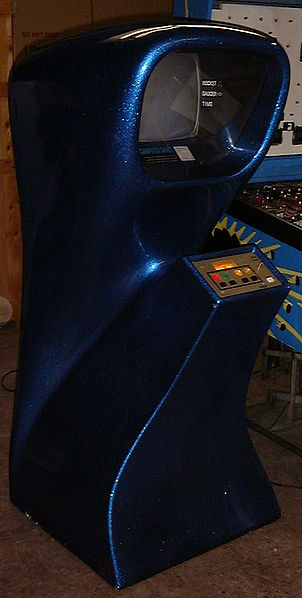
\includegraphics[scale=1.5]{computer-space.eps}}
\end{pspicture}
\bi
\item 1972: Computer Space
\item Bushnell \& Dabney 
\item Each put their \$250 into {\em Atari}
\item Dabney left to repair pinball machines
\item Bushnell stayed \& built {\em PONG}
\item Success!
\item Sued by Magnavox
\item Settled for \$750,000
\ei


\nextslide{Golden age of arcade games}
\graphic{9.5,-4}{2in}{pacman.eps}
\bi
\item 1971: {\em Computer Space} (too hard)
\item 1972: {\em PONG}, Atari, 19,000 sold
\item 1978: {\em Space Invaders}, Taito
\item 1978: {\em Asteroids}, Atari
\item 1979: {\em Pac-Man}, Namco
\ei

\nextslide{Golden age of arcade games}
\graphic{9.5,-4}{1.5in}{donkeykong.eps}
\bi
\item 1981: {\em Donkey Kong}
\item 1981: {\em Frogger}
\item 1981: {\em Galaga}
\item 1982: {\em Dig Dug}
\item 1982: {\em Q*bert}
\item 1983: {\em Dragon's Lair}
\item 1983: {\em Mario Brothers}
\ei

\nextslide{University mainframes}
\graphic{7.5,-5.5}{3in}{teletype.eps}
\bi
\item Pre 1975: Paper teletype
\item Post 1975: CRT screens
\ei

\nextslide{University mainframes, paper}
\graphicbox{9,-5}{3in}{startrek.eps}
\bi
\item 1971: {\em Computer Baseball}
\item 1971: {\em Star Trek}
\item 1972: {\em Hunt the Wumpus}
\item 1974: {\em Maze War}
\item 1975: {\em Adventure}
\ei

\nextslide{University mainframes, CRT}
\graphic{10,-4}{2in}{zork.eps}
\bi
\item 1975: {\em Dungeon}, unlicensed {\em Dungeons \& Dragons}
\item 1975: {\em dnd}
\item 1977: {\em Air}, online
\item 1977: {\em Zork}, founded Infocom
\item 1980: {\em Rogue}, random dungeons
\ei

\nextslide{Early handhelds}
\graphic{10,-4}{1in}{Microvision2.eps}
\bi
\item 1972: {\em OXO}, Waco (Toymaker)
\item 1979: {\em Microvision}, Milton-Bradley
\ei
\bigskip

LCD wasn't available until 1980's

\nextslide{Consoles: first generation}
\graphicbox{9,-4}{2in}{Pong.eps}
\graphic{2,-4}{2in}{Magnavoxodyssey.eps}
\bi
\item 1951: Ralph Baer, interactive TV idea
\item 1972: Magnavox Odyssey, \$100
\ei

\nextslide{Consoles: second generation}
\graphic{9,-5.5}{2in}{spaceinvaders.eps}
\bi
\item 1977: Atari 2600
\item 1978: Odyssey 2
\item 1979: Activision, third party developer
\item 1980: Intellivision (Mattel)
\item Atari {\em vs.} Intellivision, first console war
\item 1982: Colecovision
\ei

\nextslide{Video game crash of 1983}
\bi
\item Poor economy
\item Natural market cycle
\item Video games perceived as fad
\item Glut of poor 2600 games
\item Competition from personal computers
\item Competition from arcades
\ei

\nextslide{Third generation, 1985-1989}
\begin{pspicture}(0,0)(0,0)
\rput(9.5,-4.5){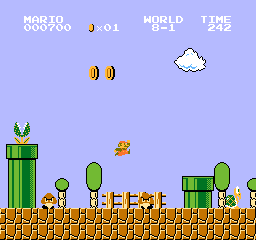
\includegraphics[width=2in]{supermariobros.eps}}
\rput(3,-6){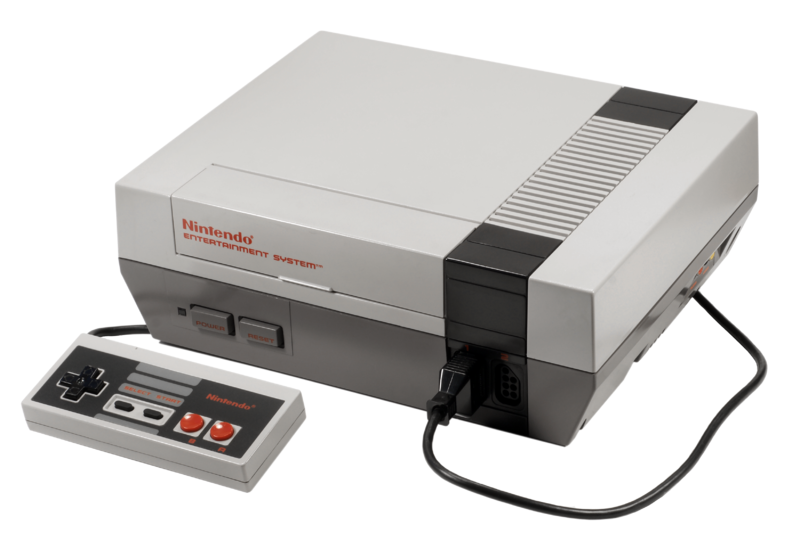
\includegraphics[width=1.5in]{nes.eps}}
\end{pspicture}
\bi
\item 1981: Nintendo {\em Donkey Kong} arcade system
\item 1985: Nintendo Entertainment System (Famicom)
\item Super Mario Bros.
\item Owned 90\% of the market
\item Introduced the gamepad
\ei

\nextslide{Third generation, 1985-1989}
\graphic{3,-5}{2in}{ffoutside.eps}
\graphic{8,-4}{2in}{ffinside.eps}
\bi
\item 1986: Dragon Quest
\item 1987: Final Fantasy
\ei

\nextslide{Home computers}
\graphic{9,-3}{2in}{appleII.eps}
\graphic{3,-5}{2in}{Commodore64.eps}
\bi
\item 1977: {\em Apple II}
\item 1981: {\em IBM PC}
\item 1982: {\em Commodore 64}\\{\small best selling computer in history}
\item 1984: {\em Apple Macintosh}
\ei

\nextslide{Home computer games}
\bi
\item Many clones of university  \& arcade games
\item Source code in books \& magazines
\item Floppies, cassettes, ROM cartridges
\ei

\nextslide{Home computer games}
\graphicbox{9,-5}{2in}{pinballconstructionset.eps}
\bi
\item 1980: {\em Zork}
\item 1980: {\em Roberta Williams Mystery House}
\item 1983: {\em Archon}
\item 1983: {\em Pinball Construction Set}
\item 1984: {\em King's Quest}
\item 1989: {\em SimCity}
\item 
\ei

\nextslide{Home computer games, 1990's}
\graphic{9,-3}{2in}{doombox.eps}
\graphic{3,-6.5}{2in}{warcraftbox.eps}
\bi
\item 1993: {\em Doom}, FPS
\item 1993: {\em Myst}
\item 1994: {\em Warcraft}, RTS
\item 1996: {\em Quake}, internet play
\ei

1996:  3d accelerator cards

\nextslide{Decline and Rebirth of Arcades}
\graphic{9,-5}{2in}{ddr.eps}
\bi
\item Home video games rival quality
\item Seedy video arcades decline
\item Family oriented video arcades arise
\item 1998: Dance Dance Revolution
\ei

\nextslide{Handhelds come of age}
\graphic{9,-2}{1in}{gameboy.eps}
\bi
\item 1989: Game Boy
\item 1990: Sega Game Gear
\ei

\nextslide{Fourth generation}
\graphic{3,-4}{2in}{sonic.eps}
\graphic{9,-4}{1.75in}{marioyoshi.eps}
\bi
\item 1988: Sega Genesis
\item 1990: SNES
\ei

\nextslide{Fifth generation}
\graphic{9,-4}{2in}{supersmashbros.eps}
3D games
\bi
\item 1994: Sega Saturn
\item 1994: Sony PlayStation
\item 1996: Nintendo 64
\ei

\nextslide{Sixth generation}
\graphic{8.5,-5.5}{3in}{grandtheftauto.eps}
\bi
\item 1998: Dreamcast
\item 2000: PlayStation 2
\item 2001: Nintendo Gamecube
\item 2001: Xbox
\ei

\nextslide{Seventh generation}
\graphic{8,-4.75}{3in}{wiisports.eps}
\bi
\item 2005: Xbox 360
\item 2006: PlayStation 3
\item 2006: Wii
  \ei

 \nextslide{Eighth generation?}
\bi
\item 2012: Wii U
\item 2012: Playstation 4
\item 2013: Xbox 720
\ei
\graphic{8,-2}{3in}{wii-u-controller.eps}

\end{slide}
\end{document}
